\chapter{Internet Protocol}
The Internet protocol was the result of research job made by american Department of Defence (DoD). \textit{Internet} means Inter-networks communication and was designed for use of interconnected systems of packet-switched computer communication networks. The only things in common between the networks is the packet architecture.\\
Today the Internet Protocol is the only one yet used in Layer 3. The Internet Protocol provides transmission of blocks of data called datagrams, from sources to destinations, where sources and destinations are hosts identified by fixed length addresses \cite{RFC791}.\\
The two main functions, that Internet Protocol needs to provide, are:
\begin{enumerate}
\item{\textbf{Definition of unified addresses (Section \ref{ip_section})}}
\item{\textbf{Fragmentation (Section \ref{fragment_section})}}
\end{enumerate}
The creation of Internet Protocol comes from the needs of interconnection between networks (Figure \ref{net_structure}). Each network has its own protocol and it's composed by serveral devices, connected each other. The terminal devices of a network are the hosts and they can talk to others in the net through routers.\\
The new devices added with the invention of Internet Protocol were the Gateways, devices similar to routers that also translate protocols of different networks. The links inside the network (that connects routers and hosts) work on Layer 3 and the links between gateways work as Layer 2 networks, that doesn't required routing function.\\
Nowadays, networks are almost local so the gateways work mostly as routers. In fact, the routers don't exist as their definition tells (Figure \ref{lan}).\\
Ping is the most known service of Internet Protocol.
\begin{figure}[h]
\centering
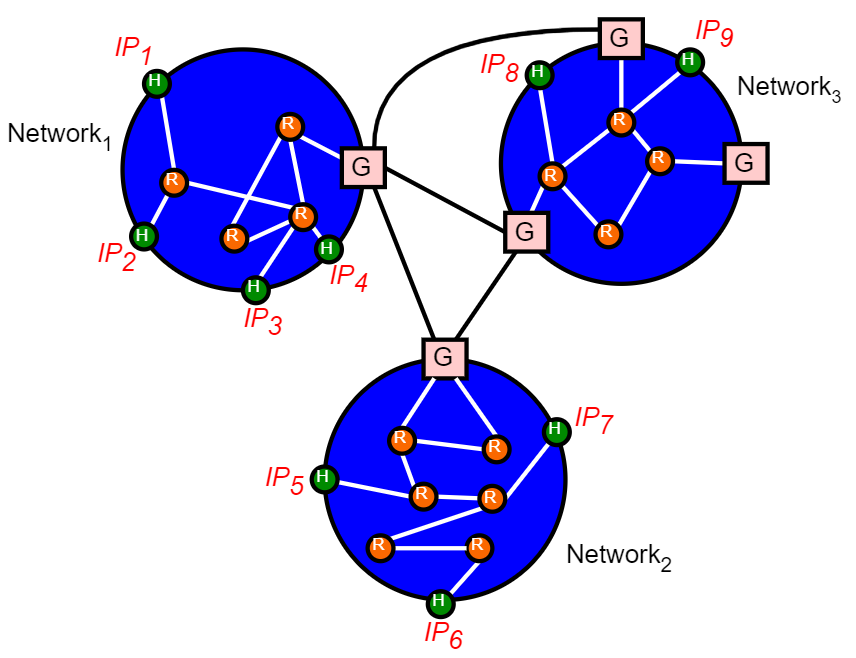
\includegraphics[scale=0.4]{Images/IP/net_structure}
\caption{\footnotesize{Internet structure.}}\label{net_structure}
\end{figure}
\begin{figure}[h]
\centering
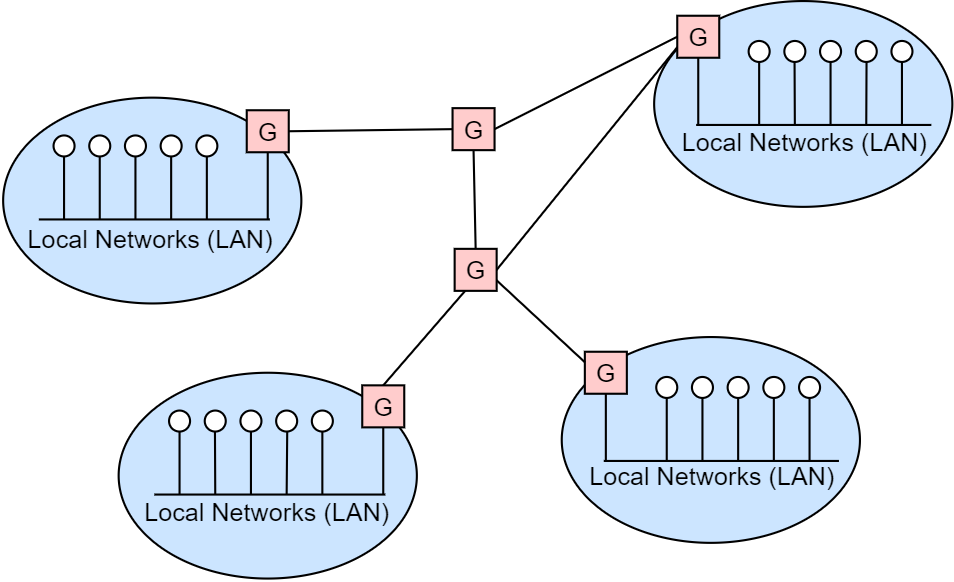
\includegraphics[scale=0.4]{Images/IP/lan}
\caption{\footnotesize{LAN structure.}}\label{lan}
\end{figure}
\clearpage
\section{Terminology}
\begin{itemize}
\item{\textbf{Round Trip Time (RTT)}\\
time needed from network to send the packet and receive the response packet
}
\item{\textbf{Delay}\\
passed time before the true service
}
\item{\textbf{Bit rate (Bandwidth)}\\
amount of Bit/s or Bytes/s of the network
}
\item{\textbf{Throughput}\\
amount of data/s that I can really transmit
}
\item{\textbf{Relaibility}\\
capacity of being reliable and losing few packets. It's related to inverse of:
$$loss\;\;rate = \frac{\#\;lost\;packets}{\#\;sent\;packets}$$
}
\end{itemize}

\section{IP address}\label{ip_section}
To send packets among different networks, we need to identify gloabally the destination host and IP address was designed to solve this problem. The IP addresses are 32 bits numbers. They are commonly represented as a set of 4 numbers separated by a point and each of them is the decimal representation of the corresponding byte in the IP address.\\
An IP address can be divided into two parts: Network part and Host part. In the past, the IP addresses were classified by three main classes, based on the size of their Network part: \textit{Class A, Class B, Class C} (Figure \ref{classes_ip}).\\
This classification of addresses in this way isn't very efficient because this cannot manage well addressing of large number of small networks or small number of large networks.\\
To do it it was introduced the Net Mask, a bit mask composed by a sequence of 1's followed by 0's, that permits us to define the parts of an address of whatever dimension we want (Figure \ref{netmask}). This is useful also to create subnetworks of a given set of hosts (Figure \ref{dei_ip}).\\
There are also two special addresses:
\begin{itemize}
\item{\textbf{Network address (no hosts)}\\
Host part = \textit{0...0000}
}
\item{\textbf{Broadcast address (all hosts in the network)}\\
Host part = \textit{1...1111}
}
\end{itemize}
Hence to give an address to each endpoint of a \textbf{Point To Point} link, we need to use at least an Host part of 2 bits (Figure \ref{point2point}).  
\begin{figure}[h]
\centering
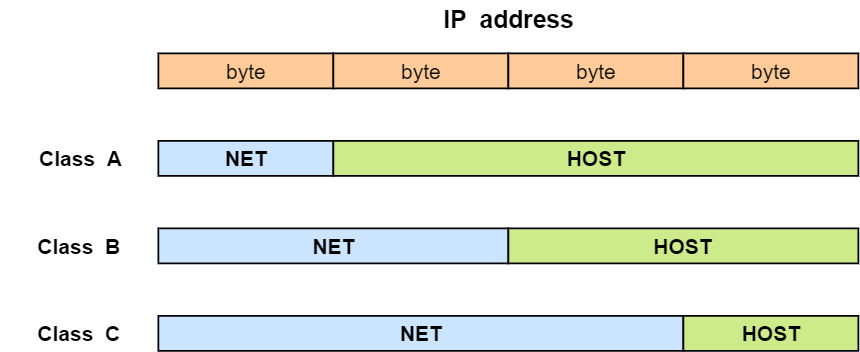
\includegraphics[scale=0.4]{Images/IP/classes_ip}
\caption{\footnotesize{IP classes.}}\label{classes_ip}
\end{figure}
\begin{figure}[h]
\centering
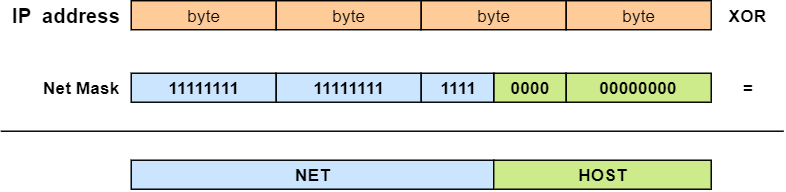
\includegraphics[scale=0.5]{Images/IP/netmask}
\caption{\footnotesize{Example of netmask use.}}\label{netmask}
\end{figure}
\begin{figure}[h]
\centering
\includegraphics[scale=0.55]{Images/IP/dei_ip}
\caption{\footnotesize{Example of subnetworks structure.}}\label{dei_ip}
\end{figure}
\begin{figure}[h]
\centering
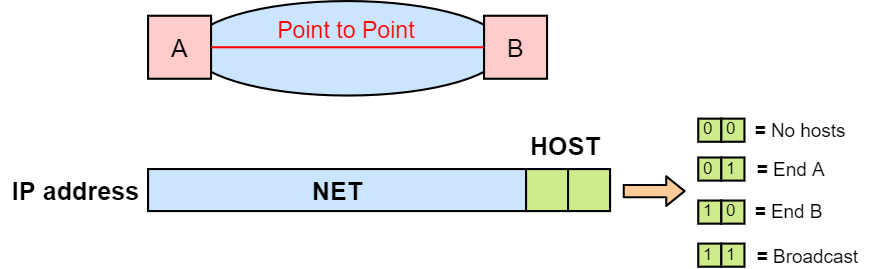
\includegraphics[scale=0.4]{Images/IP/point2point}
\caption{\footnotesize{Example of Point to Point connection network.}}\label{point2point}
\end{figure}
\clearpage
\section{Fragmentation}\label{fragment_section}
In each network, the IP information is embedded in a Layer 3 packet that respects protocol of the network in which it is. Then when the packet reach a gateway, its IP info is removed from the packet and encapsulated in a Layer 2 packet, to be sent to another network (Figure \ref{packets}). Each IP packet is also called \textbf{Datagram}.\\
Each network is defined by a Maximum Transfer Unit (MTU), that defines the maximum size of each Layer 3 packet inside the network. Hence, if the IP information, that reach a gateway of the network, is larger than MTU, the gateway reduces its size (Figure \ref{fragmentation}).\\
If a packet pass through many networks and their MTUs are very different, using datagrams, we are sure that the packets won't arrive as in the same order in which they are sent. The reason why this happens is that they are sent without the use of a stream. To manage this problem, when the gateway creates a packet, this stores the first index of the sequence of the bytes of the original IP information.\\
The last packet, that composed initial IP message, has the flag \textbf{More Fragments(MF)} set to 0. This information with the knowledge of the length and the first byte index of the last packet, permits to define the length of the original message, whenever it arrives. Each packet can fit easly in the buffer of the gateway receiver (Figure \ref{label_fragment}).
\begin{figure}[h]
\centering
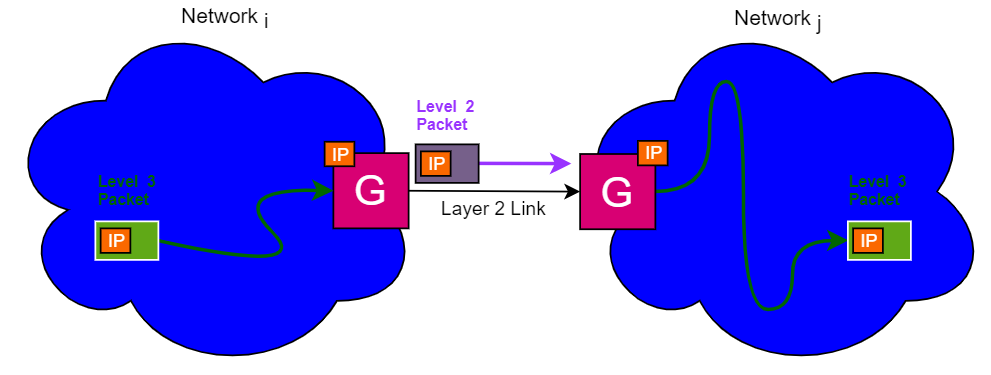
\includegraphics[scale=0.5]{Images/IP/packets}
\caption{\footnotesize{Example of encapsulation of IP packet.}}\label{packets}
\end{figure}
\begin{figure}[h]
\centering
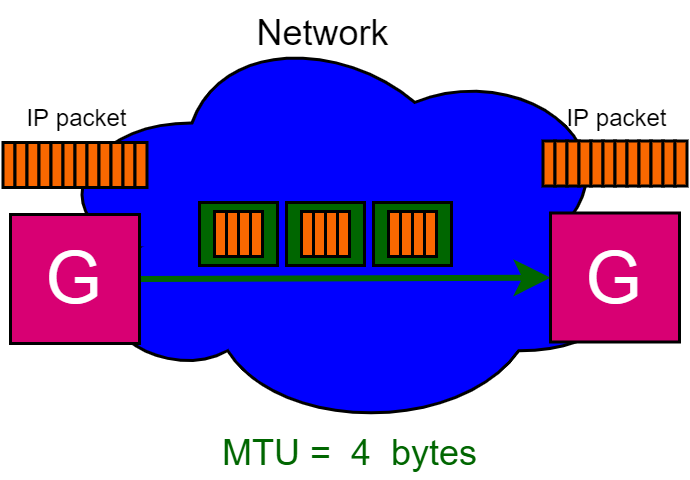
\includegraphics[scale=0.4]{Images/IP/fragmentation}
\caption{\footnotesize{Example of fragmentation.}}\label{fragmentation}
\end{figure}
\begin{figure}[h]
\centering
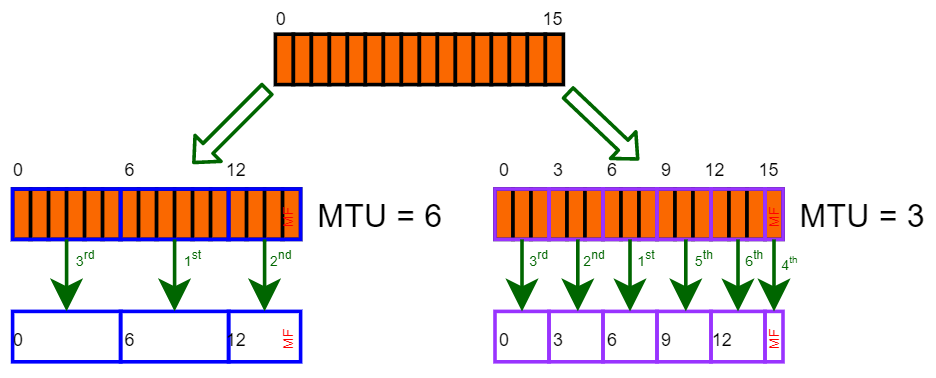
\includegraphics[scale=0.4]{Images/IP/label_fragment}
\caption{\footnotesize{Example of fragment labeling.}}\label{label_fragment}
\end{figure}

\section{Internet Header Format}
\begin{figure}[h]
\centering
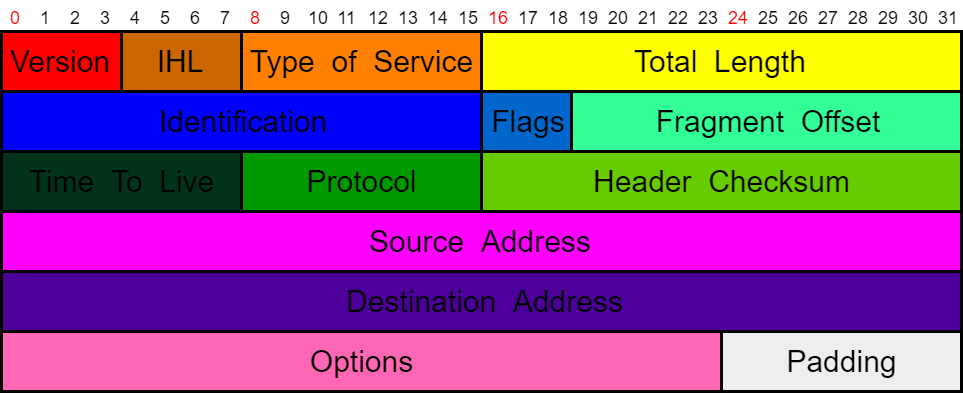
\includegraphics[scale=0.3]{Images/IP/internet_header}
\caption{\footnotesize{Internet header format.}}\label{internet_header}
\end{figure}
The content of the internet header is (Figure \ref{internet_header}):
\begin{itemize}
\item{\textbf{Version}
format of the internet header
}
\item{\textbf{IHL}\\
length, measured in words of 32 bits, of the internet header (minimum value = 5)
}
\item{\textbf{Type of Service}\\
parameters of the Quality of Service (QoS) desired (Figure \ref{flags}). Bits \textbf{6-7} are reserved for future use.
\begin{figure}[h]
\centering
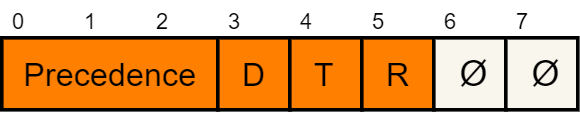
\includegraphics[scale=0.3]{Images/IP/service_type}
\caption{\footnotesize{Type of service field.}}\label{service_type}
\end{figure}
\begin{table}[h]
\centering \footnotesize
\begin{tabular}{|c|c|c|c|}
\cline{2-4}
\multicolumn{1}{c|}{}&{Delay (D)}&{Throughput(T)}&{Relaibility (R)}\\
\hline
{0}&{Normal}&{Normal}&{Normal}\\
\hline
{1}&{Low}&{High}&{High}\\
\hline
\end{tabular}
\caption{Bits 3,4,5 of Type of Service.}
\end{table}
\begin{table}[H]
\centering \footnotesize
\begin{tabular}{|c|l|}
\hline
\textbf{111}&{Network Control}\\
\hline
\textbf{110}&{Internetwork Control}\\
\hline
\textbf{101}&{CRITIC/ECP}\\
\hline
\textbf{100}&{Flash Override}\\
\hline
\textbf{011}&{Flash}\\
\hline
\textbf{010}&{Immediate}\\
\hline
\textbf{001}&{Priority}\\
\hline
\textbf{000}&{Routine}\\
\hline
\end{tabular}
\caption{Precedence of Type of Service.}
\end{table}
}
\item{\textbf{Total Length}\\
length, measured in octets, including internet header and data
}
\item{\textbf{Identification}\\
an identifying value assigned by the sender to aid in assembling the fragments of a datagram
}
\item{\textbf{Flags}\\
varius control flags. The bit 0 is reserved and must be 0.
\begin{figure}[h]
\centering
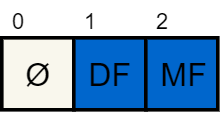
\includegraphics[scale=0.3]{Images/IP/flags}
\caption{\footnotesize{Flags.}}\label{flags}
\end{figure}
\begin{table}[H]
\centering \footnotesize
\begin{tabular}{|c|c|c|}
\cline{2-3}
\multicolumn{1}{c|}{}&{Don't Fragment (DF)}&{More Fragments (MF)}\\
\hline
{0}&{May Fragment}&{Last Fragment}\\
\hline
{0}&{Don't Fragment}&{More Fragments}\\
\hline
\end{tabular}
\caption{DF and MF flags.}
\end{table}
}
\item{\textbf{Time to Live}\\
maximum time the datagram is allowed to remain in the internet system
}
\item{\textbf{Protocol}\\
the next level protocol used in the data portion of the internet datagram
}
\item{\textbf{Header Checksum}\\
a checksum on the header only
}
\item{\textbf{Source Address}\\
the source IP address
}
\item{\textbf{Destination Address}\\
the destination IP address
}
\item{\textbf{Options}\\
it'svariable and itmay appear or not in datagrams. They must be implemented by all IP modules (host and gateways).  What is optional is their transmission in any particular datagram, not their implementation.
}
\end{itemize}